%%%%%%%%%%%%%%%%%%%%%%%%%%%%%%%%%%%%%%%%%%%%%%%%%%%%%%%%%%%%%%%%%%%%%%
% How to use writeLaTeX: 
%
% You edit the source code here on the left, and the preview on the
% right shows you the result within a few seconds.
%
% Bookmark this page and share the URL with your co-authors. They can
% edit at the same time!
%
% You can upload figures, bibliographies, custom classes and
% styles using the files menu.
%
%%%%%%%%%%%%%%%%%%%%%%%%%%%%%%%%%%%%%%%%%%%%%%%%%%%%%%%%%%%%%%%%%%%%%%

\documentclass[12pt]{article}

\usepackage{sbc-template}

\usepackage{graphicx,url}

\usepackage{chemformula} % para escrever CO2 corretamente

%\usepackage[brazil]{babel}   
\usepackage[utf8]{inputenc}  

     
\sloppy

\title{Instructions for Authors of SBC Conferences\\ Papers and Abstracts}

\author{Guilherme Fernandes Moraes da Silva\inst{1}, Daniel Cordeiro\inst{1}}

\address{Escola de Artes, Ciências e Humanidades -- Universidade de São Paulo (USP)\\ -- São Paulo, SP -- Brasil
  \email{\{guilherme.fernandes01,daniel.cordeiro\}@usp.br}
}

\begin{document} 

\maketitle

\begin{abstract}
Cloud computing has expanded its capacity through geo-distributed data centers, which, however, entail high energy consumption and increased greenhouse gas emissions. In this work, we investigate, through simulation, various scheduling algorithms applied to geo-distributed data centers with the objective of reducing environmental impact. It is expected that experiments using simulators will provide a foundation for the implementation of strategies that promote energy savings and minimize emissions.
\end{abstract}
     
\begin{resumo}
A computação em nuvem tem ampliado sua capacidade por meio de \textit{data centers} geodistribuídos, os quais, entretanto, implicam um elevado consumo energético e aumento nas emissões de gases do efeito estufa. Neste trabalho, investigamos por meio de simulação de diferentes algoritmos de escalonamento aplicados a \textit{data centers} geodistribuídos, com o objetivo de reduzir o impacto ambiental. Espera-se que os experimentos com simuladores forneçam subsídios para a implementação de estratégias que promovam a economia de energia e a minimização das emissões.
\end{resumo}


\section{Introdução}
Atualmente, os \textit{data centers} representam aproximadamente 1\% do consumo energético global e, juntamente com as redes de transmissão de dados, respondem por cerca de 1\% das emissões de gases do efeito estufa associadas à energia, fenômeno potencializado pelos expressivos aumentos no armazenamento e na carga de trabalho desses centros \cite{masanet:20}. Segundo a International Energy Agency (IEA), os dois maiores consumidores de energia do mundo -- China e Estados Unidos -- registraram elevações na demanda energética impulsionadas pelo crescimento dos \textit{data centers}. Em 2024, esses países foram responsáveis por mais da metade do consumo energético global. Projeções\footnote{https://www.iea.org/reports/electricity-2025} indicam que, na China, o consumo de energia dos \textit{data centers} poderá dobrar até 2027. Já nos Estados Unidos, os \textit{data centers} consumiram 176 TWh em 2023, representando 4,4\% do consumo total do país, com estimativas\footnote{https://eta-publications.lbl.gov/sites/default/files/2024-12/lbnl-2024-united-states-data-center-energy-usage-report.pdf} sugerindo que esse valor pode crescer para uma faixa entre 325 e 580 TWh em 2028, correspondendo de 6,7\% a 12\% do consumo total do país.

Uma estratégia promissora para mitigar as emissões de gases do efeito estufa nos \textit{data centers} consiste no desenvolvimento de algoritmos de escalonamento eficientes, voltados para a minimização dessas emissões. Para tal, simuladores são amplamente utilizados, pois oferecem uma plataforma controlada que possibilita a modelagem precisa do comportamento dos sistemas. Essa abordagem permite testar diferentes cenários e configurações, avaliando o impacto de diversos algoritmos de escalonamento e facilitando a implementação de melhorias que otimizem o desempenho e a sustentabilidade das instalações.

Diante desse contexto, este trabalho propõe a realização de experimentos com simuladores para identificar e avaliar algoritmos, ou combinações destes, que possam superar as soluções atualmente disponíveis, com o objetivo de reduzir o impacto ambiental por meio da minimização das emissões de gases do efeito estufa.

\section{Desafios em simulações cientes de emissões} \label{sec:firstpage}

Os simuladores constituem uma ferramenta fundamental para o estudo de sistemas distribuídos, pois permitem reproduzir em ambiente virtual o comportamento de plataformas de grande escala, mitigando os custos e riscos associados a testes em infraestruturas reais. Além de oferecer resultados confiáveis -- corroborados por ampla validação científica --, esses simuladores facilitam a exploração de cenários de difícil acesso prático, bem como a redução de gastos em tempo, dinheiro e energia.

Quando se busca incorporar a análise de emissões de \ch{CO2}, surgem desafios adicionais. A modelagem do consumo energético requer dados e componentes específicos, capazes de distinguir entre fontes renováveis e não renováveis ou de mensurar o impacto de estratégias de escalonamento na eficiência energética. É frequente a necessidade de módulos externos ou adaptações nos simuladores para avaliação ambiental.

Comparar algoritmos de escalonamento é uma tarefa complexa, pois cada solução pode privilegiar aspectos distintos -- como latência, qualidade de serviço, custo, consumo de energia ou emissões de \ch{CO2} --, adotando modelos e métricas próprias \cite{kumar:19}. Além disso, o fato de esses algoritmos poderem ser testados em diferentes simuladores torna ainda mais difícil obter resultados diretamente comparáveis. Nesse contexto, \textit{frameworks} como o SimGrid \cite{casanova:14} fornecem uma base flexível, centrada em aplicações distribuídas, que pode ser estendida com módulos de análise de emissões. Tal abordagem facilita a investigação de novas estratégias voltadas à otimização de recursos e à redução de impactos ambientais em \textit{data centers}.

\section{CD-ROMs and Printed Proceedings}

In some conferences, the papers are published on CD-ROM while only the
abstract is published in the printed Proceedings. In this case, authors are
invited to prepare two final versions of the paper. One, complete, to be
published on the CD and the other, containing only the first page, with
abstract and ``resumo'' (for papers in Portuguese).

\subsection{Subsections}

The subsection titles must be in boldface, 12pt, flush left.

\section{Figures and Captions}\label{sec:figs}


Figure and table captions should be centered if less than one line
(Figure~\ref{fig:exampleFig1}), otherwise justified and indented by 0.8cm on
both margins, as shown in Figure~\ref{fig:exampleFig2}. The caption font must
be Helvetica, 10 point, boldface, with 6 points of space before and after each
caption.

\begin{figure}[ht]
\centering
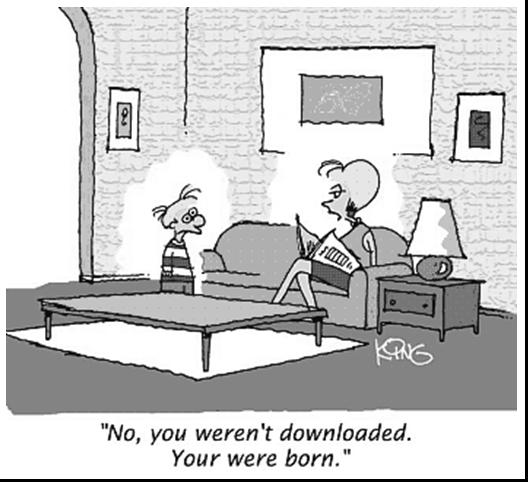
\includegraphics[width=.5\textwidth]{fig1.jpg}
\caption{A typical figure}
\label{fig:exampleFig1}
\end{figure}

\begin{figure}[ht]
\centering
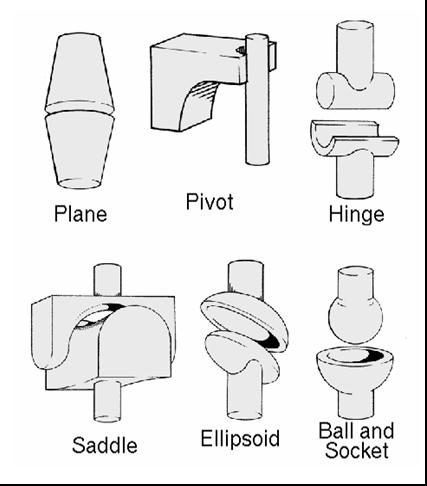
\includegraphics[width=.3\textwidth]{fig2.jpg}
\caption{This figure is an example of a figure caption taking more than one
  line and justified considering margins mentioned in Section~\ref{sec:figs}.}
\label{fig:exampleFig2}
\end{figure}

In tables, try to avoid the use of colored or shaded backgrounds, and avoid
thick, doubled, or unnecessary framing lines. When reporting empirical data,
do not use more decimal digits than warranted by their precision and
reproducibility. Table caption must be placed before the table (see Table 1)
and the font used must also be Helvetica, 10 point, boldface, with 6 points of
space before and after each caption.

\begin{table}[ht]
\centering
\caption{Variables to be considered on the evaluation of interaction
  techniques}
\label{tab:exTable1}
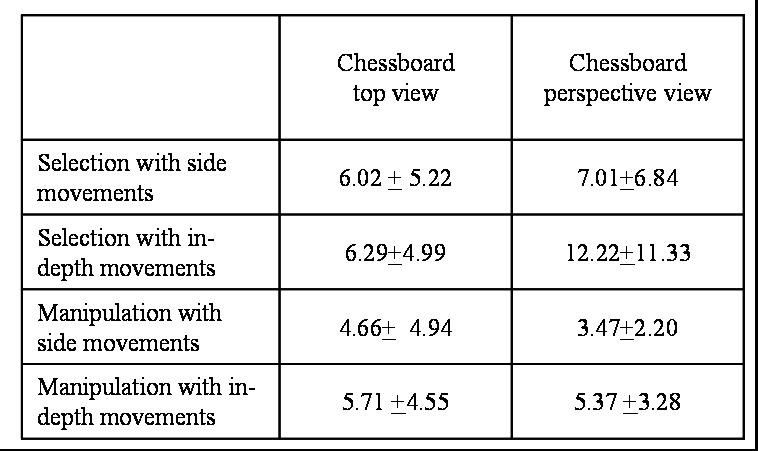
\includegraphics[width=.7\textwidth]{table.jpg}
\end{table}

\section{Images}

All images and illustrations should be in black-and-white, or gray tones,
excepting for the papers that will be electronically available (on CD-ROMs,
internet, etc.). The image resolution on paper should be about 600 dpi for
black-and-white images, and 150-300 dpi for grayscale images.  Do not include
images with excessive resolution, as they may take hours to print, without any
visible difference in the result. 

\section{Referências}

\bibliographystyle{sbc}
\bibliography{sbc-template}

\end{document}
